% WWW 2027 research-track submission (8 pages + references + appendix, double-blind).
% Revision of 12 October 2026: spatial and temporal correlation are the theoretical core.
% Theory sources: research/gpt_sol_10_09 (synthesis + spatiotemporal appendix),
% research/alignment_paper, research/correlated_arms. Evidence: research/claude_opus_10_12_v3.
% Compile:  tectonic -X compile main.tex
\documentclass[sigconf,review,anonymous]{acmart}

\usepackage{booktabs}
\usepackage{mathtools}
\settopmatter{printacmref=false}
\setcopyright{none}
\renewcommand\footnotetextcopyrightpermission[1]{}
\acmConference[WWW '27]{The ACM Web Conference 2027}{May 10--14, 2027}{Dublin, Ireland}

\newtheorem{prediction}{Prediction}
\newcommand{\E}{\mathbb{E}}
\newcommand{\Var}{\mathrm{Var}}
\newcommand{\Cov}{\mathrm{Cov}}
\newcommand{\diag}{\operatorname{diag}}
\newcommand{\I}{\mathcal{I}}
\setlength{\emergencystretch}{1.5em}

\begin{document}

\title{When Can a Bandit Trust Correlation?\\Spatial and Temporal Dependence in Web Bandits}

\author{Anonymous Author(s)}
\affiliation{\institution{Submission to the Research Track}\country{}}

\begin{abstract}
Web rewards are correlated in space and time. Items that are close in a co-engagement or hyperlink graph share long-run appeal and short-run shocks, and engagement persists for days. We develop a theory of bandits under this spatiotemporal dependence and test its predictions on three Web platforms. Each reward is a fixed long-run mean plus an autoregressive deviation whose innovations are correlated across arms. A graph can play two distinct roles: it can restrict the means through a Laplacian energy bound, or shape the shock covariance. We show that the node-time covariance factors into a spatial innovation covariance and per-arm temporal impulse responses, and is separable only when all arms share the same dynamics. An exact innovation regression turns any adaptive, restless history into a predictable linear experiment. Its information is bounded above and below by sample counts scaled by the extremes of the spectral density, which combines the shocks' spatial spectrum with the AR frequency response. This yields graph-regularized confidence sets valid at all times and sublinear mean regret. In graph Fourier modes, long-run information is $c^2/q_k$ per field, so graph-smooth shocks make rough contrasts cheap and smooth ones expensive. Certified graph pooling remains valid under this dependence. Confidence sets built for independent rewards are inflated by the autocorrelation under bursty exposure, and the best sampling schedule depends on how spatial correlation meets the lag structure. On real data, held-out Wikipedia attention shows the predicted inflation, a week of views carrying the information of 1.3--1.9 independent days, and iid certificates fail in 56--95\% of runs on worlds calibrated to it. Certified pooling gains track the components it can reject (Spearman $-0.87$ on KuaiRec, $-0.81$ on the Open Bandit Dataset), and persistence-aware policies halve regret on a chronological KuaiRec panel.
\end{abstract}

\begin{CCSXML}
<ccs2012>
<concept><concept_id>10010147.10010257.10010282.10010284</concept_id>
<concept_desc>Computing methodologies~Online learning settings</concept_desc><concept_significance>500</concept_significance></concept>
<concept><concept_id>10002951.10003317.10003347.10003350</concept_id>
<concept_desc>Information systems~Recommender systems</concept_desc><concept_significance>300</concept_significance></concept>
</ccs2012>
\end{CCSXML}
\ccsdesc[500]{Computing methodologies~Online learning settings}
\ccsdesc[300]{Information systems~Recommender systems}
\keywords{multi-armed bandits, spatiotemporal dependence, graph bandits, restless bandits, autoregressive rewards, confidence sequences}

\maketitle

%=====================================================================
\section{Introduction}
%=====================================================================

Every day a short-video platform fills a trending slot, and its rewards are correlated in two ways. \emph{Spatially}, videos that are close in a co-engagement graph tend to share long-run appeal, and a shock such as a holiday or a community event hits related videos together. \emph{Temporally}, a video's engagement today predicts its engagement for days. Classical bandits assume neither. Graph bandits assume the first, as a static restriction on means~\cite{valko2014spectral,ban2021local}. Restless and autoregressive bandits assume the second, usually with independent arms~\cite{chen2023autoregressive,trella2025latent}. This paper studies both together: what each kind of correlation does to the information in an observation, to the validity of confidence sets, and to regret.

\paragraph{Relevance to the Web.} Spatiotemporal dependence is the normal state of Web rewards. The graphs are by-products of logging (co-engagement, embeddings, hyperlinks), not priors designed for the decision. Attention persists and spreads along those graphs. Exposure is bursty, because the same items fill a slate day after day. An online learner on a Web platform must therefore decide which correlation it can trust and how much each observation is worth. We answer with theory, and test it on KuaiRec short video~\cite{gao2022kuairec}, Wikipedia attention, and the Open Bandit Dataset~\cite{saito2021obd}.

\paragraph{Two ways to go wrong.} A learner can trust spatial correlation that is not there: pooling along a graph whose neighbourhoods do not share appeal biases estimates and can cause linear regret. Or it can ignore temporal correlation: confidence sets built for independent rewards are too narrow when consecutive observations move together, so irrevocable decisions such as dropping an item go wrong. The theory below explains when each failure occurs and what repairs it.

\paragraph{Contributions.}
\begin{enumerate}
\item \textbf{A spatiotemporal reward model with two graph roles} (\S\ref{sec:model}). A graph may restrict the long-run means or shape the innovation covariance. These are different assumptions, and only the first identifies unobserved arms. The node-time covariance factors into spatial and temporal parts, and it is separable only under homogeneous dynamics (Proposition~\ref{prop:cov}).
\item \textbf{Information under spatiotemporal dependence} (\S\ref{sec:info}). An exact innovation regression gives graph-regularized confidence valid at all times under any adaptive restless schedule. A spectral sandwich bounds its information using the shock spectrum and the AR frequency response, and yields sublinear mean regret. Long-run information decomposes by graph Fourier mode. Two exact results show the interaction between space and time. Contrasts gain from correlated shocks even under staggered sampling. In an AR(2) example, block schedules beat alternation because spatial correlation is reachable only at informative lags.
\item \textbf{Certified pooling across space under persistence in time} (\S\ref{sec:pool}). Certified pooling's regret depends on which components the certificate makes rejectable, and graph geometry beyond diameters sets its information cost. Pooling stays valid under persistent, correlated shocks when built on the innovation regression (B1). Confidence built for independent rewards fails under bursty exposure by a temporal inflation factor (B2). All geometric constants carry over with the long-run covariance (B3).
\item \textbf{Predictions tested on three platforms} (\S\ref{sec:evidence}). The tests cover dose-response across certificates, real against rewired graphs, inflation in held-out Wikipedia attention predicted by its fitted autocovariance, certificate validity on real-calibrated dynamics, the slate contrast gain, and persistence on a chronological KuaiRec panel.
\end{enumerate}

%=====================================================================
\section{A spatiotemporal reward model}\label{sec:model}
%=====================================================================

There are $N$ arms. Arm $i$'s reward field is
\begin{equation}\label{eq:model}
X_{i,t}=\mu_i+z_{i,t},\qquad z_{i,t}=\sum_{r=1}^{p_i}a_{i,r}z_{i,t-r}+\eta_{i,t},\qquad \eta_t\stackrel{\rm iid}{\sim}N(0,Q_G).
\end{equation}
In round $t$ the learner chooses $a_t$, or a slate of $k$ arms, before seeing the field, and observes $Y_t=X_{a_t,t}+\xi_t$ with $\xi_t\sim N(0,r)$. Every arm evolves every round (restless), but only chosen arms are observed. The means $\mu$ are fixed and unknown. The AR polynomials $A_i(s)=1-\sum_ra_{i,r}s^r$ are stable, and $c_i=A_i(1)$, so the raw AR intercept is $c_i\mu_i$. For the theory, the orders, coefficients, $Q_G$ and $r$ are known; \S\ref{sec:evidence} tests estimated dynamics.

\paragraph{Spatial correlation: two roles for a graph.} A graph with Laplacian $L_\mu$ may restrict the \emph{means}: $\mu^\top L_\mu\mu\le S^2$ and $\|\mu\|\le B$. This is deterministic side information, and through effective resistance it implies component widths, $|\mu_i-\mu_j|\le S\sqrt{(e_i-e_j)^\top L_\mu^\dagger(e_i-e_j)}$. A graph with Laplacian $L_\eta$ may instead shape the \emph{shocks}, for example $Q_G\propto(\alpha_\eta I+\lambda_\eta L_\eta)^{-1}$ rescaled to given variances. One graph may serve both roles, but that is an additional assumption. The roles also differ in identification. Correlated shocks improve prediction and comparisons, but they cannot identify the mean of an arm that is never observed: its column of the design is zero, so $\mu_i$ does not enter the likelihood. Only a mean restriction links an unobserved arm to observed ones.

\paragraph{Temporal correlation and its interaction with space.} Stack each arm's current deviation and lags into $s_t$. Then $s_{t+1}=Fs_t+E\eta_{t+1}$ and $z_t=Cs_t$, where $F$ is block-diagonal with the AR companion blocks, $E$ inserts innovations, and $C=E^\top$. The stationary state covariance solves $\Gamma=F\Gamma F^\top+EQ_GE^\top$. Although $F$ is block-diagonal, $EQ_GE^\top$ couples the arms.

\begin{proposition}[Node-time covariance]\label{prop:cov}
Let $G_h=\Cov(z_{t+h},z_t)=CF^h\Gamma C^\top$, and write
\[
z_{i,t}=\textstyle\sum_{k\ge0}\psi_i(k)\eta_{i,t-k}
\]
with impulse response $\psi_i$. Then
\[
(G_h)_{ij}=(Q_G)_{ij}\sum_{k\ge0}\psi_i(k+h)\psi_j(k),
\]
and the spectral density matrix is
\[
\mathcal S_z(\omega)=\Lambda(\omega)\,Q_G\,\Lambda(\omega)^*,\qquad \Lambda(\omega)=\diag\big(A_i(e^{-{\rm i}\omega})^{-1}\big).
\]
The covariance is a fixed spatial matrix times a scalar temporal kernel if and only if all arms have the same impulse response. Otherwise $G_h$ is generally asymmetric for $h>0$.
\end{proposition}

The innovation covariance supplies the spatial coupling, and each pair of filters sets its lag profile. Consequences follow directly. An AR(20) arm can have no lag-1 correlation but strong lag-20 correlation. Two arms can be uncorrelated at lag 1 and correlated at lag 2. A lag-1 summary, such as a single persistence parameter, therefore misstates the information in a schedule (Proposition~\ref{prop:ar2}).

\paragraph{Regret.} \emph{Mean regret} $R_\mu(T)=\sum_t(\mu^\star-\mu_{a_t})$ measures learning of persistent appeal. \emph{Dynamic regret} $\sum_t(\max_iX_{i,t}-X_{a_t,t})$ measures tracking against an oracle that sees the current field. Actual-reward regret against the best fixed arm can be negative, because adaptive policies exploit predictable positive deviations: $\E R_{\rm fixed}=\E R_\mu-\sum_t\E z_{a_t,t}$. Several familiar models are special cases. iid bandits have $p_i=0$ and diagonal $Q_G$. Graph bandits add only the mean restriction. Restless AR bandits have no mean restriction.

%=====================================================================
\section{Information under spatiotemporal dependence}\label{sec:info}
%=====================================================================

\paragraph{The innovation regression.} Conditional on a candidate $\mu$, a Kalman filter~\cite{kalman1960} tracks $s_t\mid\mu,\mathcal H_t\sim N(g_t+D_t\mu,P_t)$, where $g_t$, $D_t$ and $P_t$ do not depend on $\mu$. For arm $a$, let $\ell_a=C^\top e_a$, $d_{t,a}=\ell_a^\top P_t\ell_a+r$ and $u_{t,a}=(e_a+D_t^\top\ell_a)/\sqrt{d_{t,a}}$.

\begin{theorem}[Predictable innovation experiments]\label{thm:innov}
The chosen observation satisfies $R_t:=(Y_t-\ell_{a_t}^\top g_t)/\sqrt{d_{t,a_t}}=u_t^\top\mu+\epsilon_t$, where $u_t=u_{t,a_t}$ is predictable and $\epsilon_t\mid\mathcal H_t,a_t\sim N(0,1)$. The online information $\I_T=\sum_tu_tu_t^\top$ and score $q_T=\sum_tu_tR_t$ equal those of the dense trajectory likelihood $Y\sim N(M\mu,\Xi)$ on every recorded path, where $\Xi$ is assembled from $G_h$.
\end{theorem}

Spatial correlation enters $u_t$ through $D_t$. Removing the predictable shared noise from a reading of arm $j$ also subtracts part of the mean of every recently observed arm, so a reading measures a weighted \emph{contrast}, not $\mu_j$ alone. Temporal correlation enters through the propagation by $F$. The mean restriction enters as a penalty, $H=\alpha I+\lambda L_\mu$, $J_T=H+\I_T$ and $\hat\mu_T=J_T^{-1}q_T$.

\begin{theorem}[Graph-regularized confidence, valid at all times]\label{thm:conf}
Suppose $\mu^\top L_\mu\mu\le S^2$, $\|\mu\|\le B$, and the graph is fixed before measurement. Let
\[
\beta_T=\sqrt{\log\tfrac{\det J_T}{\det H}+2\log\tfrac1\delta}+\sqrt{\alpha B^2+\lambda S^2}.
\]
Then, with probability at least $1-\delta$, $|v^\top(\hat\mu_T-\mu)|\le\beta_T\|v\|_{J_T^{-1}}$ for all $T$ and all contrasts $v$ simultaneously. Stopping when every comparison with the leader clears its width returns the best arm with probability at least $1-\delta$.
\end{theorem}

The first term of $\beta_T$ prices the stochastic error after whitening in space and time~\cite{abbasi2011improved}. The second prices the spatial restriction. If the graph is only approximately right, $(1-\zeta)L_\mu\preceq\hat L\preceq(1+\zeta)L_\mu$, replacing $S^2$ by $(1+\zeta)S^2$ keeps the guarantee. That repair applies only to the mean role. A shock covariance fitted from the wrong graph changes the likelihood itself.

\begin{proposition}[Spectral information sandwich]\label{prop:sandwich}
Let $a_{\min}$ and $a_{\max}$ be the extremes of $|A_i(e^{-{\rm i}\omega})|$ over arms and frequencies, and set $v_\pm=\lambda_{\max/\min}(Q_G)/a_{\min/\max}^2+r$. For every realized schedule, $v_+^{-1}\diag(N_i(T))\preceq\I_T\preceq v_-^{-1}\diag(N_i(T))$, where $N_i(T)$ is the number of observations of arm $i$.
\end{proposition}

The worst-case information per observation is $1/v_+$, which combines the largest spatial eigenvalue of the shocks with the most persistent temporal frequency. For AR(1), $a_{\min}=1-\varphi$, which recovers the $(1-\varphi)^{-2}$ cost of persistence that appears in B1 below.

\begin{corollary}[Sublinear mean regret]\label{cor:ucb}
Mean-UCB on $\hat\mu_i+\beta_{t-1}\sqrt{(J^{-1})_{ii}}$, with forced cyclic probes at square ages ($F_T\le N+\sqrt T$), has, with probability at least $1-\delta$,
\begin{gather*}
R_\mu(T)\le2BF_T+4\beta_T\sqrt{v_+NT},\\
\beta_T\le\sqrt{N\log\big(1+\tfrac{T}{\alpha v_-}\big)+2\log\tfrac1\delta}+\sqrt{\alpha B^2+\lambda S^2}.
\end{gather*}
\end{corollary}

This bound is conservative. Its value is that it holds under arbitrary spatial and temporal correlation. Sharper constants require the long-run structure below.

\begin{proposition}[Long-run information and graph modes]\label{prop:lr}
Observing the full field for $n\ge p$ rounds gives $\I_n=\I_p+(n-p)D_cQ_G^{-1}D_c$ with $D_c=\diag(c_i)$. The sample-mean field has long-run covariance $\mathcal K_{\rm LR}=D_c^{-1}Q_GD_c^{-1}=\mathcal S_z(0)$. If all arms share coefficients ($D_c=cI$) and $Q_G$ shares eigenvectors $\phi_k$ with $L$, eigenvalues $q_k$ and $\ell_k$, then the information about the graph mode $\phi_k^\top\mu$ grows as $nc^2/q_k$, and a penalty $\lambda L$ adds $\lambda\ell_k$.
\end{proposition}

This is the spectral form of the interaction between space and time. Persistence ($c\to0$) scales every mode's information by $c^2$. Graph-smooth shocks, such as $Q_G=(\alpha_\eta I+\lambda_\eta L)^{-1}$ with $q_k^{-1}=\alpha_\eta+\lambda_\eta\ell_k$, cancel in rough contrasts. High-frequency differences between neighbours are therefore cheap to learn. The global level ($\ell_1=0$), which no contrast reveals, is the most expensive. The mean penalty also acts on high frequencies, so the two graph roles reinforce each other only on rough modes.

\begin{proposition}[Temporal inflation of iid confidence, B2]\label{prop:b2}
If arm $i$ is observed in blocks of $b$ consecutive rounds, its sample-mean variance is inflated by $f_i(b)=1+2\sum_{h<b}(1-h/b)\rho_i(h)$, where $\rho_i(h)=(G_h)_{ii}/(G_0)_{ii}$. For AR(1) this is $\frac{1+\varphi}{1-\varphi}-\frac{2\varphi(1-\varphi^b)}{b(1-\varphi)^2}$. An iid radius $\sqrt{2\sigma^2\ell/n}$ then miscovers with per-check probability $2\Phi(-\sqrt{2\ell/f_i(b)})$.
\end{proposition}

By Proposition~\ref{prop:cov}, $\rho_i$ depends only on arm $i$'s own filter. Within-arm inflation is purely temporal, while every contrast between arms is spatiotemporal:

\begin{proposition}[Contrasts, B3(2)]\label{prop:contrast}
Two arms observed together $n$ times have long-run contrast variance $(\Omega_{ii}+\Omega_{jj}-2\Omega_{ij})/n$, where $\Omega=\mathcal K_{\rm LR}$ is restricted to the observed pair. With common dynamics, this is $Q_{SS}/c^2$ for the observed set $S$; it is not the full-field precision restricted to $S$. With equal variances, the gain over independent shocks is the factor $1-\rho$. Under staggered observation, lag-one cross-covariances replace the lag-zero ones. Under persistence these are nearly equal, so the gain survives, whereas under iid rewards it vanishes.
\end{proposition}

\begin{proposition}[Space meets lag: an exact schedule comparison]\label{prop:ar2}
Let two arms follow $z_{i,t}=az_{i,t-2}+\eta_{i,t}$ with stationary variance $V$ and innovation correlation $\rho$. For four observations with noise $r$, the GLS contrast variance is $V+r-a\rho V$ under the schedule AABB and $V+r+aV$ under ABAB. AABB therefore has strictly higher fixed-mean probability of correct selection for every gap.
\end{proposition}

Alternation looks natural for comparing two arms, but here it is wrong. Under AABB, each arm's consecutive readings are independent (lag 1), while readings of different arms two rounds apart share the correlated shock (lag 2). ABAB does the reverse: it reaches within-arm redundancy and misses the cross-arm correlation. At $V=1$, $r=0.1$, $a=0.8$, $\rho=0.6$ and gap $0.4$, the variances are 0.62 and 1.90, and the probabilities of correct selection are 0.694 and 0.614. No single persistence number can rank these schedules. The ranking requires the spatial and temporal structure together, as in Proposition~\ref{prop:cov}.

%=====================================================================
\section{Certified pooling across space under persistence in time}\label{sec:pool}
%=====================================================================

\paragraph{Spatial pooling with iid noise.} SP-UCB partitions the arms into components $C_c$ with certified widths $\varepsilon_c$. It keeps arm bounds $u_i=\bar Y_i+b(n_i)$ and pooled bounds $\hat p_c+b(N_c)+\varepsilon_c$, selects the component that maximizes the minimum of its two bounds, $U_c$, and pulls that component's best arm. SP-KLUCB uses KL radii~\cite{garivier2011klucb}. Let $v_c=\max_{i\in C_c}\mu_i$, let $\Gamma_c=\mu^\star-v_c$ be the component gap, and let $\ell=\log(2(N+M)T/\delta)$.

\begin{theorem}[A1: alignment-sensitive regret]\label{thm:a1}
With valid widths, with probability at least $1-\delta$,
\[
\mathcal R_T\le\textstyle\sum_{c\in\mathcal O}A_c+\sum_{c\notin\mathcal O}\min\{A_c,H_c\}.
\]
Here $\mathcal O$ is the set of components containing an optimal arm, $A_c=\sum_{i\in C_c:\Delta_i>0}(\Delta_i+8\sigma^2\ell/\Delta_i)$ is the cost of arm-by-arm exploration, and $H_c=(\Gamma_c+\varepsilon_c)(1+8\sigma^2\ell/(\Gamma_c-\varepsilon_c)^2)$ is the cost of rejecting the whole component. $H_c$ is finite only when the component is \emph{rejectable}, that is, when $\varepsilon_c<\Gamma_c$.
\end{theorem}

Widths do not capture all of the graph's information. For a suboptimal component of $m$ arms with gap $\Delta$ and energy radius $S$, the structured lower bound~\cite{combes2017minimal} has constant $C_{L,S}=2\sigma^2/(\Delta F_L^*(S/\Delta))$, where $F_L^*\in[1/m,1]$ is the value of a graph-energy design problem (Appendix~\ref{app:proofs}). Its sensitivity to the supplied uncertainty is set by the \emph{resistance radius} $\rho_L$, the radius of the smallest enclosing ball in the effective-resistance embedding: $C_{L,S}\Delta/2\sigma^2=1+2(S/\Delta)\rho_L+O((S/\Delta)^2)$. A clique and a path with the same resistance diameter differ sharply. At $S=\Delta$,
\[
C_{\rm clique}=\frac{2\sigma^2m}{\Delta},\qquad C_{\rm path}\le\frac{2\sigma^2}{\Delta(1-1/\sqrt2)^2},
\]
with no factor of $m$ for the path. Without a certificate, pooling is unsafe. For $\mu=(1,0.9,0)$ with arms 1 and 3 linked, smoothing makes arm 2 look best (failure N1). This needs an informative graph, because a random graph shrinks all arms uniformly and preserves rankings.

\paragraph{Adding temporal dependence.} Build both bounds from Theorem~\ref{thm:innov}: $U_i=\hat\mu_i+\beta_t\|e_i\|_{J_t^{-1}}$, and the component bound
\[
U_c=\min_{w\in\Delta(C_c)}\big(w^\top\hat\mu+\beta_t\|w\|_{J_t^{-1}}\big)+\varepsilon_c.
\]

\begin{theorem}[B1: certified pooling under spatiotemporal dependence]\label{thm:b1}
With valid widths and correctly specified dynamics, every arm and component bound holds at all rounds with probability at least $1-\delta$, under any adaptive restless schedule and any $Q_G$. If each pull from component $c$ adds at least $\iota$ to the realized information of its best weighted contrast, Theorem~\ref{thm:a1} holds with $8\sigma^2\ell$ replaced by $4\beta_T^2/\iota$. For independent AR(1) arms, $\iota\ge(1-\varphi)^2/(V+r)$.
\end{theorem}

A pooled component's information is the sum of its arms' information, so its per-pull increase has the same lower bound $\iota$; it does not grow by a factor of $|C_c|$. The rejection condition $\min_w\|w\|^2_{J_t^{-1}}\ge(\Gamma_c-\varepsilon_c)^2/4\beta_t^2$ holds for every schedule. The log-determinant in $\beta_T$ costs a factor of $\sqrt N$. Scalar constructions avoid it. With diagonal $Q_G$, each statistic is a scalar martingale (B1$'$). With correlated shocks, the other arms' means enter as bounded nuisances, and plugging in intervals that contain the truth preserves validity when iterated from $[0,1]$ (B1$''$). The price of correlation is visible in the nuisance terms $\sum_{j\ne i}|G_{ij}|\rho_j$, which couple every interval to every other.

\begin{proposition}[B3(1): long-run constants]\label{prop:b3}
Under long runs or full slates, every constant of the mean channel ($A_c$, $H_c$ and $C_{L,S}$) holds with $\sigma^2$ replaced by the long-run variance $\mathcal K_{\rm LR}$. With common coefficients this is $q/c^2$, and for AR(1) it is $V(1+\varphi)/(1-\varphi)$. Contrast constants use Proposition~\ref{prop:contrast}.
\end{proposition}

The two dependencies therefore act on different parts of the regret bound. Space decides which components are rejectable and at what geometric cost. Time rescales every constant by the long-run variance, and it decides whether iid confidence sets are even valid.

\begin{prediction}\label{pred:all}
(a) Certified gains rise with the share of rejectable components, across certificates and platforms. (b) Uncertified pooling fails on informative graphs, never on rewired ones, and real graphs beat rewirings only through rejectability. (c) iid certificates fail under bursty exposure at the rate given by $f(b)$, and innovation certificates do not. (d) Real attention shows the inflation that the full autocovariance predicts, and lag-1 summaries miss it. (e) Correlated shocks help when several arms are compared at once. (f) Persistence-aware policies beat iid policies, and exploring the fresh innovation is wasted.
\end{prediction}

%=====================================================================
\section{Evidence}\label{sec:evidence}
%=====================================================================

\subsection{Spatial structure of the mean (a, b)}

\paragraph{Design.} KuaiRec's 1,411 users $\times$ 3,327 videos matrix is 99.6\% observed, and a larger, disjoint log lets us build 16 graphs without leakage (Appendix~\ref{app:data}). Collaborative graphs carry taste: factorization and co-engagement neighbours agree on double-centred taste at 17--23 times the random-pair level (Table~\ref{tab:align}). Tag, category, profile and location graphs mostly encode popularity, or nothing. In Setting A, each of 120 held-out users $\times$ 3 subsets (360 instances) gets 300 videos, each item graph is rebuilt on them, SP-KLUCB uses a 20-component spectral partition, and $T=20{,}000$. Ratios are to KL-UCB at the same fixed level.

\begin{table}[t]\centering\small
\setlength{\tabcolsep}{3pt}
\begin{tabular}{lcccc}
\toprule
Certificate (I-mf graph) & Regret ratio & 90th pct. & Valid & Rejectable \\
\midrule
Oracle widths & \textbf{0.64} [0.61, 0.67] & 1.04 & 100\% & 59\% \\
Per-user calibrated, q75 & 0.82 & 1.04 & 74\% & -- \\
Population calibrated, q50 & 0.70 [0.66, 0.73] & 1.04 & 47\% & 62\% \\
Population calibrated, q90 & 0.99 [0.98, 0.99] & 1.04 & 90\% & 15\% \\
Energy (from the graph) & 0.96 [0.95, 0.97] & 1.04 & 100\% & 21\% \\
None (zero width) & 0.37 [0.35, 0.40] & 1.08 & 0\% & 95\% \\
\bottomrule
\end{tabular}
\caption{Certified pooling on KuaiRec (360 instances). Regret ratio: ratio of mean regrets to KL-UCB, with 95\% CI. The 90th percentile is of per-instance ratios. Valid: share of components whose width covers the true range. Rejectable: share of suboptimal components with width below their gap.}\label{tab:certgap}
\end{table}

\begin{figure}[t]\centering
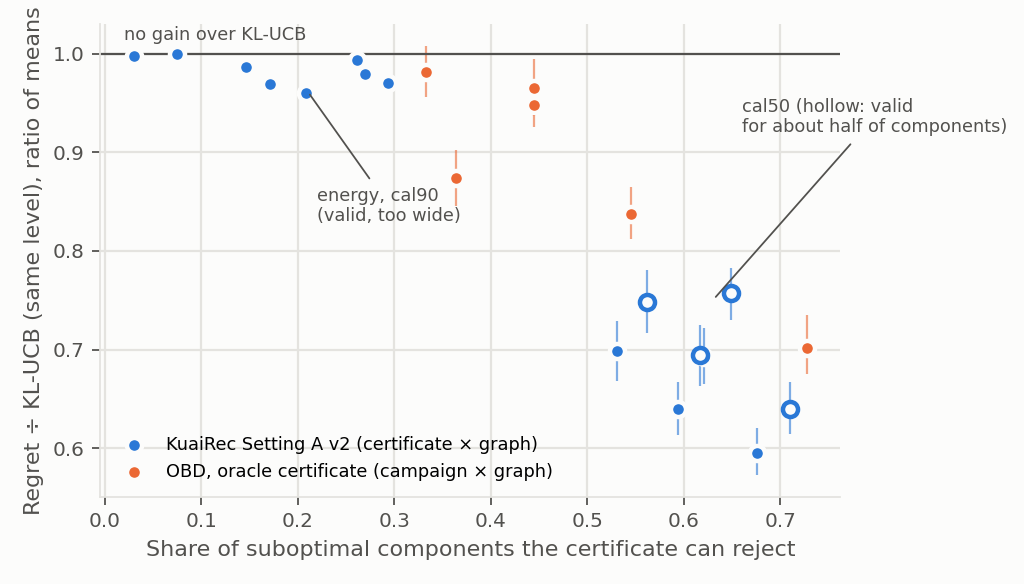
\includegraphics[width=0.92\linewidth]{figures/r1_dose_response.png}
\caption{Gains track the share of components the certificate can reject (Theorem~\ref{thm:a1}). Points are certificate $\times$ graph cells on KuaiRec and campaign $\times$ grouping cells on the Open Bandit Dataset. Hollow points are certificates valid for under 85\% of components.}\label{fig:dose}
\end{figure}

\paragraph{Findings.} Across the 16 certificate $\times$ graph cells, regret falls as the rejectable share rises (Spearman $-0.87$; Figure~\ref{fig:dose}). Valid but wide certificates (energy, q90) reject 15--29\% of suboptimal components and gain 1--4\%. The oracle rejects 59--68\% and gains 30--40\%. The per-instance link is weak ($-0.09$), so rejectability predicts which certificate helps better than which instance it helps. Zero-width pooling is best on average but carries the tail. Spectral TS on co-engagement averages 1.54$\times$ TS, with 27\% of users above 2$\times$. Failures occur on informative graphs and never on rewired ones (N1). Paired over the 360 instances, oracle pooling on the real factorization graph has $0.916\times$ the regret it has on the rewired graph [0.905, 0.926], because the real graph makes more components rejectable (59\% against 53\%). Uncertified pooling (1.03) and spectral TS (1.00) cannot be told apart from the null, and graph-free shrinkage is the best average policy. On the Open Bandit Dataset, with item click rates as means and components from a held-out prefix, all three findings replicate. The rank correlation over six cells is $-0.81$, uncertified pooling on audience clusters never finds the best item and its regret grows linearly, and empirical-Bayes TS is best (0.21--0.29$\times$ KL-UCB). \emph{Spatial structure in the means pays only through certified rejection.}

\subsection{Temporal dependence and certificates (c, d)}

\paragraph{Controlled worlds.} We use 20 arms in four components of five, with widths 0.1. Deviations are AR(1) with $\varphi\in\{0,0.5,0.9,0.97\}$, with independent shocks or shocks correlated along a path. Exposure is one arm at a time, or blocks of 25 consecutive rounds as in a daily slate, with $T=5{,}000$.

\begin{table}[t]\centering\small
\setlength{\tabcolsep}{3.5pt}
\begin{tabular}{ccccc}
\toprule
$\varphi$ & $\sqrt{f(25)}$ (B2) & iid violated & B1$''$ violated & iid drops best arm \\
\midrule
0 & 1.00 & 0\% & 0\% & -- \\
0.5 & 1.68 & 0\% & 0\% & -- \\
0.9 & 3.49 & 85\% & 0\% & 28\% (batch 25), 39\% (100) \\
0.97 & 4.42 & 90--95\% & 0\% & 72\% (batch 25), 89\% (100) \\
\bottomrule
\end{tabular}
\caption{B2's predicted inflation against observed failures (blocks of 25). Drops: certified successive elimination, 100 worlds per cell, $T=20{,}000$; valid elimination never dropped the best arm. With one-at-a-time exposure, iid certificates were never violated.}\label{tab:b2}
\end{table}

\paragraph{Findings.} Violations follow $f(b)$ (Table~\ref{tab:b2}). One-at-a-time UCB interleaves arms, so repeat pulls are about 20 rounds apart and the inflation stays small. Innovation certificates had no violations in 2,080 runs with known dynamics, and 0--3\% in later sweeps ($\delta=0.05$). With dynamics fitted on a 365-round prefix there were 0/60 violations, and a 100-round prefix gave 13\%. The dangerous misspecification is a missed lag. Fitting AR(1) when the truth has a weekly AR(7) lag gives 23\% violations, as Proposition~\ref{prop:cov} warns (Figure~\ref{fig:validity}, Appendix Table~\ref{tab:robust}). Once iid elimination drops the best arm, regret grows linearly at 0.14--0.26 per round. Validity has a price, though. At $\varphi\ge0.9$, valid elimination removes nothing within 20,000 rounds, which is the $(1-\varphi)^{-2}$ factor of Proposition~\ref{prop:sandwich}.

\begin{figure}[t]\centering
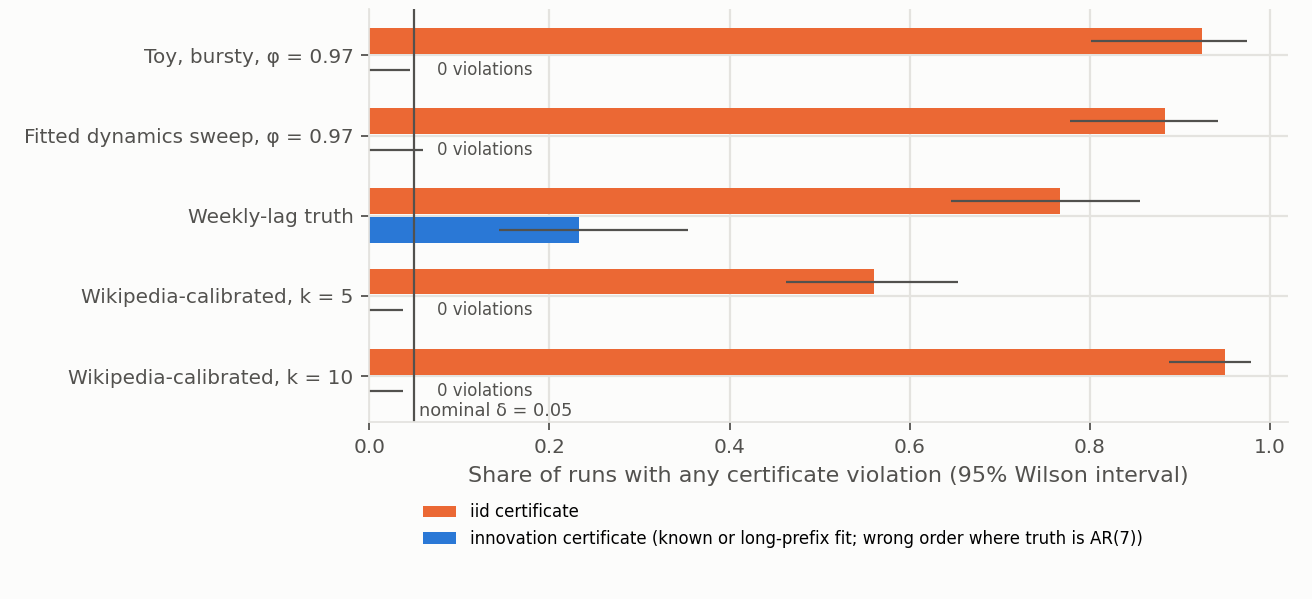
\includegraphics[width=0.92\linewidth]{figures/r3_validity.png}
\caption{Share of runs with any certificate violation (95\% Wilson intervals): the toy model, the estimated-dynamics sweep, a weekly-lag truth fitted as AR(1), and worlds calibrated to Wikipedia attention with slates of $k$ articles.}\label{fig:validity}
\end{figure}

\paragraph{Real attention.} For 300 Wikipedia articles, we fit $\log(1+\text{views})$ on 2022--2023 and measure block-mean variance on 2024--2025. Weekday-adjusted, a 7-day block has 5.0--5.3 times the variance of seven independent days, and a 28-day block 17--18 times. A week of exposure therefore carries the information of 1.3--1.9 independent days. The full autocovariance of an AR(20) fit predicts held-out inflation to within 4--23\%, while the lag-1 shortcut underpredicts by a factor of 1.2--3.3 (Table~\ref{tab:inflation}). This is Proposition~\ref{prop:b2} with the whole of $\rho_i(h)$. On 730-day worlds calibrated to 30 articles (AR(7) dynamics, real residuals, slates of 5 or 10), iid certificates are violated in 56\% and 95\% of runs, while innovation certificates are violated in 0--1\%, including with re-fitted dynamics. They are too wide to act on, however. After two years the pointwise posterior width is 0.07, inside the 0.135 gap, but the log-determinant ellipsoid reaches 0.70, and the B1$''$ plug-in reaches 1.74 because shocks correlated across 30 arms couple every interval (Figure~\ref{fig:widths}). The missing piece is a per-contrast anytime bound paying $\sqrt{\log\log n}$~\cite{howard2021confidence} after whitening in space and time.

\begin{table}[t]\centering\small
\setlength{\tabcolsep}{3pt}
\begin{tabular}{lcccc}
\toprule
Panel & Block & Observed & AR(1) from $\rho(1)$ & AR(20), full ACF \\
\midrule
One domain & 7 days & 5.0 & 3.4 & 4.5 \\
One domain & 28 days & 17.1 & 4.6 & 13.2 \\
Six communities & 7 days & 5.3 & 4.4 & 5.0 \\
Six communities & 28 days & 17.8 & 7.4 & 15.3 \\
\bottomrule
\end{tabular}
\caption{Inflation $f(b)$ of block means in Wikipedia attention: medians over 150 articles, weekday-adjusted, observed in 2024--2025 against predictions from 2022--2023 fits.}\label{tab:inflation}
\end{table}

\begin{figure}[t]\centering
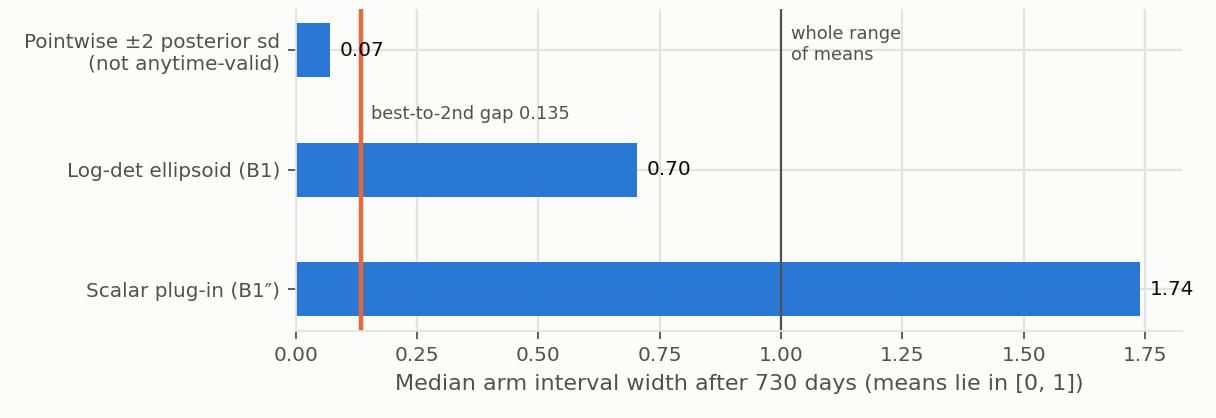
\includegraphics[width=0.92\linewidth]{figures/r5_widths.png}
\caption{Median arm interval width after 730 days on Wikipedia-calibrated dynamics with the true model. The information is there, but the anytime-valid constructions do not exploit it.}\label{fig:widths}
\end{figure}

\subsection{Spatial shocks and persistence in decisions (e, f)}

\paragraph{Exact checks.} We computed Proposition~\ref{prop:contrast} exactly and confirmed it by Monte Carlo (within 0.3\%). With $\varphi=0.9$ and $n=365$, contrast variance relative to $\rho=0$ is 0.70, 0.40 and 0.10 at $\rho=0.3$, 0.6 and 0.9. Unequal variances or dynamics shrink the gain, to 0.28--0.38 at $\rho=0.9$. Staggered observations keep 96--99\% of the gain under persistence and none under iid rewards. In a 100-arm grid with AR(20) dynamics and grid-correlated shocks, joint predictive sampling cuts dynamic regret by 29\% against TS. Correlated shocks add 15\% beyond persistence alone, and the gain vanishes with independent shocks (Appendix Table~\ref{tab:toy}).

\paragraph{KuaiRec daily slot, chronologically.} The panel covers 63 days. At each cutoff the co-engagement graph is rebuilt from earlier interactions only. There are three disjoint 11-day test windows crossed with five panels of 49--50 videos, budgets of $k=1$ and 5, and hyperparameters frozen after a development window.

\begin{table}[t]\centering\small
\setlength{\tabcolsep}{3pt}
\begin{tabular}{lcc}
\toprule
Policy (regret $\div$ iid Thompson sampling) & $k=1$ & $k=5$ \\
\midrule
Joint filter, greedy & \textbf{0.47} [0.25, 0.70] & 0.44 [0.35, 0.52] \\
Last observed value & 0.49 [0.28, 0.74] & \textbf{0.43} [0.31, 0.55] \\
Temporal-only filter, greedy & 0.50 & 0.46 \\
Joint filter, UCB & 0.51 [0.30, 0.73] & 0.46 [0.38, 0.54] \\
\quad rewired graph / common factor only & 0.50 / 0.50 & 0.47 / 0.48 \\
Sliding-window UCB & 0.61 & 0.74 \\
Discounted Thompson sampling & 0.77 & 0.90 \\
\bottomrule
\end{tabular}
\caption{KuaiRec daily slot, chronological protocol: regret per slot per day relative to iid TS (15 panel-window units).}\label{tab:chrono}
\end{table}

\paragraph{Findings.} Persistence pays: the joint filter cuts regret by 49--56\% against iid TS (Table~\ref{tab:chrono}), and standard discounting~\cite{garivier2011switching} is clearly worse. The last observed value matches it; the difference is inconclusive, at $+3\%$ and $+7\%$. Spatial shocks help only when several arms are compared at once, as Proposition~\ref{prop:contrast} predicts. At $k=5$ the shock covariance cuts regret by 11\% [5\%, 20\%] against the temporal-only filter, and at $k=1$ it does nothing. Most of that gain comes from a common factor, so the prefix graph cannot be distinguished from its rewiring. Exploring the fresh innovation is wasted. Current-state TS is the worst learning policy both in the grid and on KuaiRec, as the identity $\Sigma-Q_G\succeq0$ (Appendix~\ref{app:proofs}) predicts.

%=====================================================================
\section{Related work}\label{sec:related}
%=====================================================================

\paragraph{Spatial dependence.} Spectral bandits assume means smooth on a graph and bound regret by an effective dimension~\cite{valko2014spectral,kocak2020spectral}. Graph pure exploration prices similarity in samples~\cite{thaker2022graph}. Clustered and collaborative bandits pool across users or arms~\cite{gentile2014clustering,carlsson2021clustered,ban2021local,wu2016collaborative}, and Web systems use social, knowledge and key-term graphs~\cite{zhao2022knowledge,wu2020graphneural,zhang2020conversational,li2025evoi}. Correlated-arm UCB pulls non-competitive arms $O(1)$ times when correlations are known~\cite{gupta2021correlated}, and network spillover adds dependence across users~\cite{faruk2025spillover}. These works use the graph in one role, with independent noise. We separate its role for the means from its role for the shocks, certify the first, and price the second in the spectral domain.

\paragraph{Temporal dependence.} Switching and drifting bandits forget old data~\cite{garivier2011switching,bogunovic2016tvgp,wu2019dynamic}. AR rewards~\cite{chen2023autoregressive}, latent AR states~\cite{trella2025latent} and linear Gaussian systems with Kalman prediction~\cite{gornet2024restless} model persistence. Predictive sampling targets information that persists~\cite{liu2023predictive}, and the knowledge gradient handles correlated beliefs~\cite{frazier2009kg}. TV-GP-UCB combines spatial and temporal kernels, but they are separable~\cite{bogunovic2016tvgp}. We credit these works for filtering and for the policies. Our contribution is the non-separable node-time structure, the information and confidence it implies, and its interaction with certified spatial pooling.

\paragraph{Confidence and evaluation on Web logs.} Self-normalized bounds~\cite{abbasi2011improved} and time-uniform confidence sequences~\cite{howard2021confidence} underlie our certificates. Off-policy conclusions on the Open Bandit Dataset are fragile, partly because its logs violate i.i.d.\ assumptions~\cite{korovaitceva2026ips}, which matches B2. Related uses of logged Web data include offline-online learning~\cite{li2021unifying}, slate evaluation~\cite{kiyohara2024slate}, empirical-Bayes ranking~\cite{yang2024empirical,wang2021hybrid}, and audits of feed exploration~\cite{vombatkere2024tiktok,li2010linucb,jia2021pairrank}.

%=====================================================================
\section{Conclusion and limitations}\label{sec:conclusion}
%=====================================================================

Spatial and temporal correlation act on different parts of a bandit's information. Space, through the mean restriction, decides which alternatives can be rejected and at what geometric cost. Through the shocks, it makes rough contrasts cheap and leaves global levels expensive. Time rescales every constant by the long-run variance, and it decides whether iid confidence is valid at all. Their interaction is not separable, and the best schedule depends on both. On the data, spatial structure in means pays only through certified rejection, real attention is in the regime where iid confidence fails, and persistence halves regret. \emph{Limitations.} The theory assumes known dynamics; our estimated-dynamics results are empirical. KuaiRec and Open Bandit Dataset means are estimated, so the mean-channel evidence is model-based on real parameters. Our Wikipedia shock panels are retrospective. The main open problem is an anytime-valid certificate that is efficient per contrast under correlated persistent shocks.

\bibliographystyle{ACM-Reference-Format}
\bibliography{references}

\appendix

%=====================================================================
\section{Proofs}\label{app:proofs}
%=====================================================================

\paragraph{Proposition~\ref{prop:cov}.} With $z_{i,t}=\sum_k\psi_i(k)\eta_{i,t-k}$ and $\Cov(\eta_{i,t},\eta_{j,s})=(Q_G)_{ij}1\{t=s\}$, we get $\Cov(z_{i,t+h},z_{j,t})=\sum_{k,k'}\psi_i(k)\psi_j(k')(Q_G)_{ij}1\{t+h-k=t-k'\}=(Q_G)_{ij}\sum_{k'}\psi_i(k'+h)\psi_j(k')$. Fourier transforming gives $\mathcal S_z$. If $\psi_i=\psi$ for every arm, then $G_h=Q_G\,\gamma(h)$ with $\gamma(h)=\sum_k\psi(k+h)\psi(k)$, which is separable. Conversely, separability makes $(G_h)_{ij}/(Q_G)_{ij}$ independent of $(i,j)$ for every $h$, so every diagonal pair $(i,i)$ has the same autocorrelation. A stable causal AR filter normalized to $\psi_i(0)=1$ is determined by its autocorrelation through spectral factorization, so all arms share one filter.

\paragraph{Theorem~\ref{thm:innov}.} Given $\mu$, the selected conditional mean is $\ell_a^\top g_t+(e_a+D_t^\top\ell_a)^\top\mu$ with variance $d_{t,a}$, so standardization gives $\epsilon_t\sim N(0,1)$. The Kalman update with gain $k_t=P_t\ell_{a_t}/d_{t,a_t}$ keeps the state mean affine in $\mu$: $D_t^+=D_t-k_tv_{t,a_t}^\top$ and $D_{t+1}=FD_t^+$. Propagation by $F$ preserves this form, and $P_t$ does not depend on $\mu$. The transform to innovations is triangular, with unit Jacobian, so it whitens $\Xi$, and the dense likelihood factors into these terms. The actions are non-anticipating, so $u_t$ is predictable.

\paragraph{Theorem~\ref{thm:conf}.} For fixed $\theta$, $\exp(\theta^\top W_T-\theta^\top\I_T\theta/2)$ with $W_T=\sum u_t\epsilon_t$ is a nonnegative martingale. Mixing $\theta\sim N(0,H^{-1})$, as a proof device rather than a prior, gives $\sqrt{\det H/\det J_T}\exp(\|W_T\|^2_{J_T^{-1}}/2)$. Ville's inequality bounds it by $1/\delta$ for all $T$. Since $\hat\mu_T-\mu=J_T^{-1}W_T-J_T^{-1}H\mu$ and $H\preceq J_T$, the bias term in the $J_T$ norm is at most $\sqrt{\mu^\top H\mu}\le\sqrt{\alpha B^2+\lambda S^2}$, and Cauchy--Schwarz extends the bound to any contrast. On this event every certified difference is positive at the truth, which gives the stopping claim. Under graph error, $\mu^\top\hat L\mu\le(1+\zeta)S^2$.

\paragraph{Proposition~\ref{prop:sandwich}.} The eigenvalues of $\mathcal S_z(\omega)$ lie in
\[
[\lambda_{\min}(Q_G)/a_{\max}^2,\ \lambda_{\max}(Q_G)/a_{\min}^2].
\] By Parseval's identity, the block Toeplitz covariance of any finite stretch of the field has its spectrum in the same interval. Selecting coordinates and adding $rI$ keeps $\Xi$ between $v_-I$ and $v_+I$. Hence $M^\top\Xi^{-1}M$ lies between $v_\pm^{-1}M^\top M=v_\pm^{-1}\diag(N_i)$, and by Theorem~\ref{thm:innov} this holds for $\I_T$ on every path.

\paragraph{Corollary~\ref{cor:ucb}.} On the confidence event, an ordinary action's gap is at most $2\beta_{t-1}\sqrt{(J^{-1})_{a_ta_t}}\le2\beta_{t-1}\sqrt{v_+/N_{a_t}}$ by the sandwich, and $\sum_tN_{a_t}^{-1/2}\le2\sqrt{NT}$. Forced rounds cost at most $2B$ each. The determinant bound follows from $J_T\preceq H+v_-^{-1}T\,I$.

\paragraph{Proposition~\ref{prop:lr}.} After $p$ fields, the innovation transform
\[
X_t-\textstyle\sum_k\diag(a_{\cdot,k})X_{t-k}=D_c\mu+\eta_t
\]
has a triangular Jacobian that does not depend on the parameters. Each field therefore adds $D_cQ_G^{-1}D_c$. The long-run covariance is $\mathcal S_z(0)=D_c^{-1}Q_GD_c^{-1}$. With $D_c=cI$ and $Q_G=\sum_kq_k\phi_k\phi_k^\top$, the information is $nc^2\sum_kq_k^{-1}\phi_k\phi_k^\top$, and adding $\lambda L=\lambda\sum_k\ell_k\phi_k\phi_k^\top$ gives the stated modes.

\paragraph{Propositions~\ref{prop:b2} and~\ref{prop:contrast}.} The variance of a block sum is $\sum_{s,u}(G_{|s-u|})_{ii}=(G_0)_{ii}\,b\,f_i(b)$. Blocks separated by other arms' blocks are nearly independent, so the sample mean is Gaussian with variance $(G_0)_{ii}f_i(b)/n$. For a contrast, $\Var(\sum_t(z_{i,t}-z_{j,t}))/n^2\to(\Omega_{ii}+\Omega_{jj}-2\Omega_{ij})/n$ with $\Omega=\sum_hG_h=\mathcal S_z(0)$. Observing only $S$ gives the marginal $Q_{SS}$, not $((Q^{-1})_{SS})^{-1}$, because the unobserved contemporaneous coordinates are not conditioned on. Staggering replaces $G_0$ by $G_1$ in the cross terms.

\paragraph{Proposition~\ref{prop:ar2}.} Odd-lag covariances vanish, and $G_{2k}=a^kV\left(\begin{smallmatrix}1&\rho\\\rho&1\end{smallmatrix}\right)$. Under AABB, each arm's two readings are one round apart and so independent, while cross-arm pairs two rounds apart have covariance $a\rho V$. The per-arm means are the GLS estimates, with contrast variance $V+r-a\rho V$. Under ABAB, each arm's readings are two apart, with covariance $aV$, and cross-arm pairs are at odd lags, which gives $V+r+aV$. For two arms the probability of correct selection is $\Phi(\Delta/\sigma)$.

\paragraph{Theorem~\ref{thm:a1} and the geometry constants.} A supermartingale argument with a union bound over $N+M$ processes and $n\le T$ gives the confidence event. On it, $v_c-\varepsilon_c\le B_{c,N_c}\le v_c$, so both terms of $U_c$ bound $v_c$. Optimism gives $n_i\le1+8\sigma^2\ell/\Delta_i^2$, which yields $A_c$. If $\Gamma_c>\varepsilon_c$, then $N_c\le1+8\sigma^2\ell/(\Gamma_c-\varepsilon_c)^2$, with each such pull costing at most $\Gamma_c+\varepsilon_c$, which yields $H_c$. For the constants: $F_L^*(s)=\max_{p\in\Delta_m}\min_i\min\{\sum_jp_jz_j^2:z_i=1,\ z\in[0,1]^m,\ z^\top Lz\le s^2\}$ is the information-design value of the structured change-of-measure program. The resistance expansion follows by perturbing at $s=0$. For the clique, every coordinate can be raised alone, so $F^*=1/m$. For the path, putting half the weight on each endpoint gives $F^*\ge(1-1/\sqrt2)^2$. The full statements are in the supplementary material.

\paragraph{Theorem~\ref{thm:b1}.} Theorem~\ref{thm:conf} with $\lambda=0$ holds for all directions, hence for every $e_i$ and every $w\in\Delta(C_c)$, and $w^\top\mu\ge v_c-\varepsilon_c$. If $c$ is selected, then $\mu^\star\le v_c+\varepsilon_c+2\beta_t\|w\|_{J_t^{-1}}$. Information growth bounds $\min_w\|w\|^2_{J^{-1}}\le1/(\iota(N_c-1))$. For independent AR(1) arms, the coefficient of $\mu_i$ in a pull of arm $i$ is $1-\varphi^hs\ge1-\varphi$ with $s\in[0,1]$, and the predictive variance is at most $V+r$. B1$''$: let $G=J-\alpha I$. Then $q_i-\sum_{j\ne i}G_{ij}m_j=G_{ii}\mu_i+\sum_{j\ne i}G_{ij}(\mu_j-m_j)+W_i$, so given intervals that contain the truth, with half-widths $\rho_j$, the error is at most $(\sqrt{2J_{ii}\log(\sqrt{J_{ii}/\alpha}/\delta')}+\alpha+\sum_{j\ne i}|G_{ij}|\rho_j)/J_{ii}$. Induction from $[0,1]$ completes the proof.

\paragraph{Proposition~\ref{prop:b3}.} Substitute the per-field information $D_cQ_G^{-1}D_c$ of Proposition~\ref{prop:lr} for count-based information in the change-of-measure program and in the proof of Theorem~\ref{thm:a1}.

\paragraph{Predictable-state exploration.} We have $z_t=CFs_{t-1}+\eta_t$, and $\eta_t$ is independent of the past, so the forecast covariance satisfies $P=\Var(CFs_{t-1}\mid\mathcal H_t,\mu)+Q_G$, hence $P-Q_G\succeq0$. Sampling with $\Sigma$ explores $Q_G$, which no observation can reduce. Sampling with $\Sigma-Q_G$ explores only learnable uncertainty. The dynamic-regret lower bound $T\{\mathcal G(\mu,K_0)-\mathcal G(\mu,K_0-Q_G)\}$, with $\mathcal G(\mu,K)=\E\max_i(\mu_i+Z_i)$, follows from a genie that knows the past state and lacks only the fresh innovation.

%=====================================================================
\section{Data and graphs}\label{app:data}
%=====================================================================

\paragraph{KuaiRec~\cite{gao2022kuairec}.} The small matrix has 1,411 users $\times$ 3,327 videos and 4.68M interactions. The disjoint big matrix has 7,176 $\times$ 10,728 and 12.5M interactions. The reward is $\min(\text{watch ratio},5)/5$. Graphs are union $k$-NN graphs ($k\in\{5,10,20\}$), with Laplacians scaled to mean degree one, and nulls are degree-preserving rewirings. User-side signals use only non-evaluation videos, and video-side signals use only non-evaluation users.

\paragraph{Wikipedia.} We use daily user page views for 2022--2025 and hyperlinks from a 2026 snapshot. One panel has the 150 most-viewed programming-language articles. The other has six communities of 25 articles each: NFL, NBA and MLB teams, Premier League clubs, UN members and programming languages.

\paragraph{Open Bandit Dataset~\cite{saito2021obd}.} ZOZOTOWN uniform-random logs from 24--30 November 2019: the All campaign (1.37M impressions over 80 items) and the Women campaign (0.86M over 46 items).

%=====================================================================
\section{Additional results}\label{app:extra}
%=====================================================================

\begin{table}[h]\centering\small
\setlength{\tabcolsep}{2.5pt}
\begin{tabular}{llccc}
\toprule
Graph & Side & Quotient & Taste corr. & Choice cost \\
\midrule
I-mf (factorization) & item & 0.76 / 0.96 & \textbf{0.046} & 0.117 / 0.019 \\
I-coeng (co-engagement) & item & 1.10 / 1.30 & \textbf{0.034} & 0.131 / 0.037 \\
I-cat, I-tag (content) & item & 0.91 / 0.99 & 0.010 & 0.099 / 0.079 \\
U-coeng (co-engagement) & user & \textbf{0.65} / 0.79 & \textbf{0.020} & 0.284 / 0.291 \\
U-geo, U-feat, U-demo & user & 0.95--0.99 & 0.002--0.007 & 0.31--0.35 \\
\bottomrule
\end{tabular}
\caption{Spatial structure of KuaiRec means ($k=10$). Quotient: $\mu^\top L\mu$ relative to random ($\approx1$), real / rewired. Taste corr.: neighbours' double-centred taste (random: $\le0.002$). Choice cost: loss in best-choice value from $(I+10L)^{-1}$ smoothing, real / rewired.}\label{tab:align}
\end{table}

\begin{table}[h]\centering\small
\begin{tabular}{lc}
\toprule
Learner (B1$''$, blocks of 25, $\varphi=0.97$) & Runs violated \\
\midrule
Known dynamics & 0/60 \\
Fitted on a 365-round prefix & 0/60 \\
Fitted on a 100-round prefix & 8/60 (13\%) \\
\quad same, persistence $+2$ standard errors & 3/60 (5\%) \\
Correlated truth fitted as independent & 0\% \\
Student-$t$(3) shocks & 3--17\% \\
AR(7) weekly-lag truth fitted as AR(1) & 23\% \\
iid certificate & 88\% \\
\bottomrule
\end{tabular}
\caption{Certificate validity with estimated and misspecified dynamics.}\label{tab:robust}
\end{table}

\begin{table}[h]\centering\small
\setlength{\tabcolsep}{2.5pt}
\begin{tabular}{lccc}
\toprule
Policy (dynamic regret per round) & Main & Indep.\ shocks & Weak persist. \\
\midrule
ST UCB, 2 sd (tuned) & \textbf{0.850} & \textbf{0.890} & 1.856 \\
ST predictive sampling & 0.950 & 1.057 & 1.568 \\
SpectralUCB & 1.026 & 1.014 & 1.953 \\
AR predictive sampling (temporal only) & 1.121 & 1.094 & \textbf{1.525} \\
ST current-state TS & 1.258 & 1.452 & 2.246 \\
Thompson sampling & 1.329 & 1.523 & 1.675 \\
\midrule
Innovation lower bound & 0.298 & 0.323 & 1.276 \\
\bottomrule
\end{tabular}
\caption{Spatiotemporal benchmark: 100-arm grid, AR(20) with coefficients summing to 0.97, grid-correlated shocks $(I+5L)^{-1}$, $T=2{,}000$, 8 seeds.}\label{tab:toy}
\end{table}

\end{document}
